\chapter{\IfLanguageName{dutch}{Stand van zaken}{State of the art}}
\label{ch:stand-van-zaken}

% Tip: Begin elk hoofdstuk met een paragraaf inleiding die beschrijft hoe
% dit hoofdstuk past binnen het geheel van de bachelorproef. Geef in het
% bijzonder aan wat de link is met het vorige en volgende hoofdstuk.

% Pas na deze inleidende paragraaf komt de eerste sectiehoofding.

In dit hoofdstuk worden de verschillende termen die aan de InsurTech en Webscraping gebonden zijn uitvoerig besproken.

\section{InsurTech}

Allereerst wordt de term InsurTech verklaard.
InsurTech is een porte-manteauwoord van insurance en technology.
Concreet is dit het introduceren of gebruik maken van innovatieve technologie in de verzekeringswereld.
Deze innovatieve technologiën worden ontwikkeld door middel van het gebruik van apps, Big Data, machine learning, draagbare producten zoals smartwatches en andere transformatieve technologiën die processen betreffende de verzekeringswereld kunnen automatiseren of bevorderen. Deze bevorderingen kunnen werken voornamelijk op basis van het ophalen van data en deze te analyseren.
De InsurTech is in principe een specialisatie van FinTech, ofwel Financial Technology.
Terwijl FinTech zich op alle financiële technologieën focust, beperkt de InsurTech zich tot die van de verzekeringswereld.
Een duidelijk verschil is dat de FinTech onder meer ook nog over technologie in banken gaat.

InsurTech is nog vrij nieuw, zo worden er regelmatig nieuwe toepassingen ontwikkeld die de efficiëntie van een verzekeringsbedrijf bevorderen. Zo wijst een artikel van \textcite{Institute2020} erop dat de term is opgekomen rond 2010, toen de hoofdimplementatie eerder prijsvergelijkingen tussen verschillende verzekeringsmaatschappijen was. Tegenwoordig reiken de toepassingen van InsurTech veel verder dan alleen prijsvergelijkingen, zoals verzekeringsadvies bieden op basis van verzamelde data. Een ander artikel uit 2021 of \textcite{InsuranceCommissioners2021} toont aan dat InsurTech startups de voorbije decennia een geschatte 16,5 miljard dollar aan investeringen hebben verzameld en dat dit bedrag in de toekomst alleen maar zal groeien. Een literatuurstudie van \textcite{inproceedings} concludeert dat de verzekeringsmaatschappijen vooral kosten, in tijd en geld, verliezen door het analyseren van de risico’s die een klant loopt om zo de juiste verzekeringen aan te raden. Door InsurTech toepassingen is het beheren van verzekeringen en de klantencommunicatie niet alleen vergemakkelijkt, maar ook verbeterd. Wat webscraping en datamining betreft bestaat er reeds een grote variëteit aan technologie en tools. Er zal zowel voor een toepassing voor webscraping, als API gebruik gezocht worden bij het vinden van een toepassing die de klantenervaring kan bevorderen.

\subsection{De werking van verzekeringen}
Een verzekering wordt door \textcite{Trowbridge1975} omschreven als een risico-overdracht waarbij
een klant het risico overdraagt aan een verzekeringsmaatschappij in ruil voor een overeengekomen bedrag. 
Het doel van de klant in dat geval is de negatieve financiële gevolgen te beperken van een onzekere toekomstige gebeurtenis.
\graphicspath{ {./img/} }
\begin{figure}[H]
	\centering
	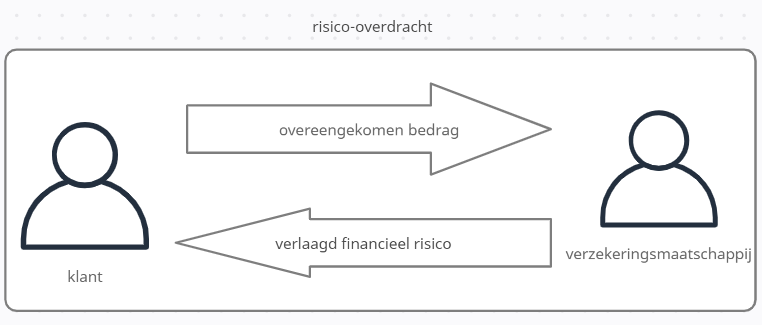
\includegraphics{creately_basic_verzekering}
	\caption{Verzekering visualisatie volgens \textcite{Trowbridge1975}}
\end{figure}
Een verzekering krijgt volgens \textcite{cortis2019insurtech} verder ook de taak en verantwoordelijkheid een inschatting te maken over welk bedrag opgesteld moet worden. Dit is afhankelijk van de grootte van het risico die de verzekeringsmaatschappij met zich meedraagt. Wanneer een klant zijn vergoeding opeist, wordt bij de verzekering een claim management proces opgesteld. Dit is opnieuw één van de processen waar tijd- en kost-efficiëntie een rol speelt.



\section{Webscraping}

Allereerst gaan we terug in de tijd, naar het ontstaan van webscraping. Webscraping dateert al van het begin van het World Wide Web, ontstaan in 1989, toen het internet voor het eerst werd geïntroduceerd. Nog geen 4 jaar later, in 1993, werd al voor het eerst de term “webscraping” gebruikt. Het jaar waarin een groep MIT (Massachusetts Institution of Technology) studenten als schoolproject de omvang van het internet probeerden in te schatten. Hun allereerste webscraper, de World Wide Web Crawler, werd de basis van vele andere webscrapers die nog in de toekomst zouden volgen. In datzelfde jaar werd alsook de allereerste zoekmachine op het internet uitgevonden door Jonathan Fletcher, de “vader van de zoekmachine”. Deze student aan de University of Sterling te Schotland ontwierp onbewust de voorloper van Google genaamd Jumpstation. \autocite{farholt2021less} Mettertijd is het gebruik van webscraping en de gebruikte toepassingen drastisch gewijzigd. Zo worden tegenwoordig webscrapers gebruikt om interactie van een gebruiker te simuleren om webpagina’s uit te testen vanuit het standpunt van de eindgebruiker.
Webscraping is reeds heel wat geëvolueerd, zo moet de technologie zich vaak aanpassen aan hoe webpagina’s eigenlijk opgebouwd zijn.
Webscraping is het extraheren en indexeren van data in webpagina’s en deze vervolgens opslaan in een tekstbestand of databank. Webpagina’s bestaan uit tekst die in verschillende formaten beschikbaar is: als gewone tekst, in tabellen, ... De simpelste vorm van webscraping is het kopiëren en plakken van tekst. Het is de taak van een webscraper om deze data automatisch uit te lezen en te indexeren. Het crawlen of scrapingsproces op het internet bestaat er allereerst uit alle gewenste data uit te lezen en om deze vervolgens in een gepast leesbaar formaat te structureren.\autocite{zhao2017web} Hoofdzakelijk wordt dit gebruikt om repetitieve taken te versnellen, zoals iedere subtitel van een pagina kopiëren en plakken. Het uitlezen kan op verschillende manieren gebeuren, afhankelijk van de desbetreffende webpagina. Echter is het niet hoofdzakelijk nodig altijd webscraping toe te passen. Soms beschikt de webpagina of service over een API, een acroniem voor Application Programming Interface. Dit is een set van functies en procedures  die één of meerdere taken vervult met als doel door software gebruikt te worden. Dit maakt het voor programmeurs makkelijker en efficiënter om net de data die men nodig heeft uit de pagina te halen zonder overbodige data ook nog in te laden. Performantiegewijs heeft het gebruik van API’s op webpagina’s of services de voorkeur. \autocite{10.2307/251584}
Abstract kan het gebruik van webscraping vanalles inhouden. Kleinschalig kan dit gaan over het monitoren van real-time data met behulp van polling, wat een detectiesysteem kan inhouden die aanpassingen op websites detecteert. Tot grootschalig het voortdurend uitlezen van website data om een zoekmachine mee te bouwen. Zo kan Google of Bing aanzien worden als één grote webscraper, gebruikt om het internet uit te mappen. \autocite{snyder2003web}

\begin{figure}[bh]
	\centering
	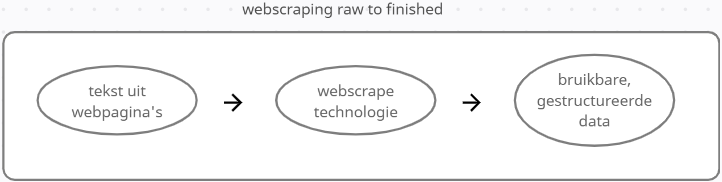
\includegraphics{webscraping_cycle}
	\caption{webscraping structuur}
\end{figure}

\subsection{Populaire Webscrapers}

% TODO leg uit waarom er gekozen werd voor enkel Selenium en puppeteer uit te leggen dmv populariteit
Om een keuze te maken tussen welke webscrapers er gekozen moet worden voor het onderzoek, moeten er vergelijkingen gedaan worden.
Wanneer de webscraping tools die binnen Python gebruikt worden worden geordend op populariteit, duidt aan dat Selenium en Puppeteer tussen de populaire webscrapers zitten. \autocite{Saurkar2018}
Ook op \href{https://trends.google.com/trends}{Google Trends} wordt aangetoond dat Selenium en Puppeteer de meest populaire zoekopdrachten staat, voor onderzoekers en ontwikkelaars.

\begin{figure}[bh]
	\centering
	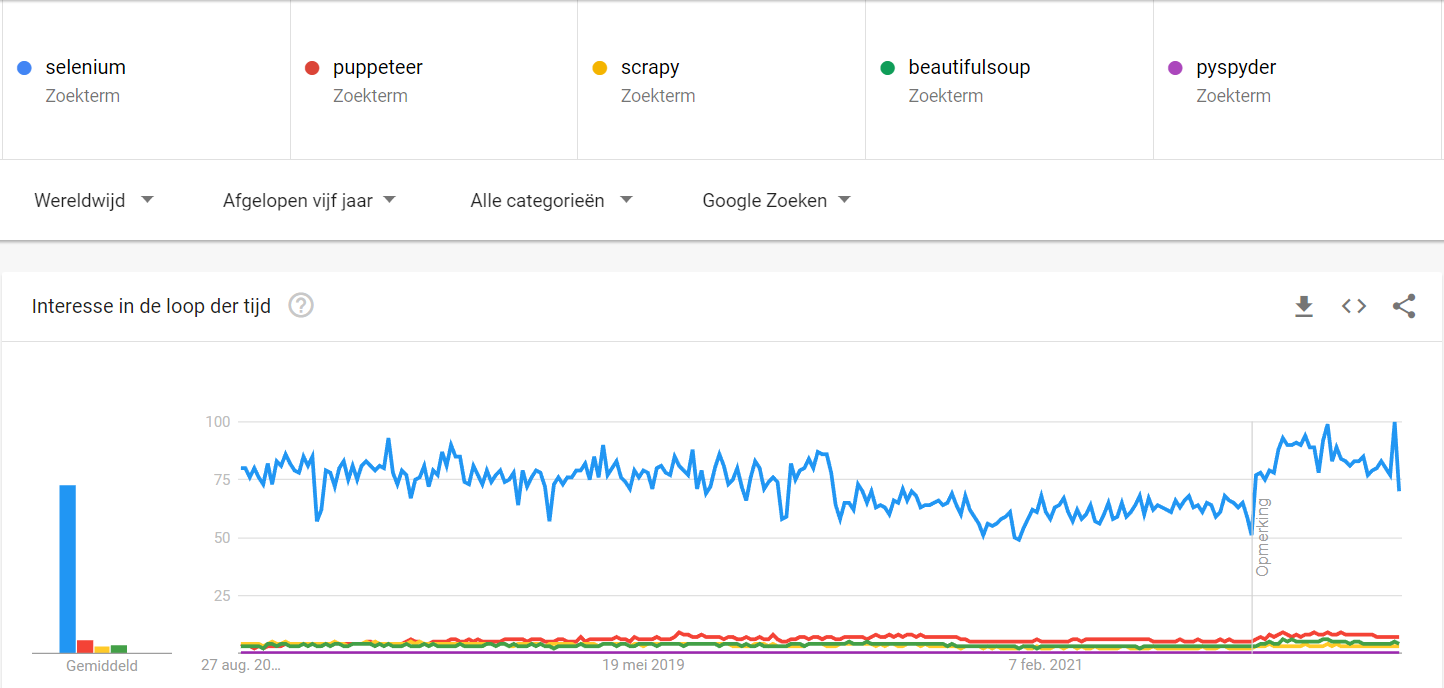
\includegraphics[width=\textwidth, height=\textheight, keepaspectratio]{python_webscrapers_google_trends}
	\caption{Vergelijking van Python webscrapers op \href{https://trends.google.com/trends}{Google Trends}}
\end{figure}

\subsection{Puppeteer}

% TODO vul aan wat Puppeteer is
Puppeteer is een library die het mogelijk maakt om een Chrome of Chromium browser te besturen vanuit code. Het besturen van de browser wordt op die manier mogelijk via een API. Deze API maakt gebruik van het DevTools protocol. Dit protocol zorgt voor tools om een browser te inspecteren, debuggen en profileren. Deze library zal echter niet gebruikt worden omdat de gekozen taal voor dit onderzoek Python is, en Puppeteer werkt op Javascript. Er is als alternatief wel een Python wrapper genaamd Pyppeteer, maar deze blijft ook eerder minder populair.

\subsection{Selenium}

Selenium is een web-UI testing library, wat wil zeggen dat de library geschikt is voor testdoeleinden. Selenium is echter niet beperkt tot deze doeleinden. Het is een set van verschillende software tools die elk een verschillende aanpak hebben om geautomatiseerde testen te ondersteunen. Het geautomatiseerd testen is de techniek van het automatiseren van de uitvoerings van testgevallen met behulp van gespecialiseerde software. Het feit dat deze library ondersteund wordt in verschillende webbrowsers maakt de library zeer toegankelijk.


\section{HTML}
De voorgaande sectie duidt op wat webscrapers precies zijn en hoe deze data ophalen, in deze sectie wordt uitgelegd uit wat deze webpagina's, waarvan webscrapers hun data halen, zijn opgebouwd.
Een website bestaat uit pagina's of documenten die tekst, afbeeldingen, stylesheets en scripts bevatten. Ze worden vaak ontwikkeld met behulp van opmaaktalen zoals Hypertext Markup Language (HTML) en Extensible Hypertext Markup Language (XHTML). HTML wordt gewoonlijk de standaard opmaaktaal genoemd die wordt gebruikt om webpagina's te genereren. Sinds het begin van de jaren negentig wordt HTML alleen gebruikt, maar soms in combinatie met servergebaseerde programmeertalen zoals PHP, ASP en JSP.  XHTML is een verbeterde en uitgebreide vorm van HTML, de standaard opmaaktaal voor online content. Ook is XHTML eenvoudiger dan HTML en is het een XML-toepassing vanuit een coderingsstandpunt. HTML specificeert en bevat de inhoud van webpagina's. Gegevensbronnen die de gegevens en informatie onthullen die kunnen worden geëxtraheerd,  kunnen in een HTML-pagina worden geplaatst binnen een vooraf gedefinieerde reeks opdrachten in opmaakcomponenten die tags worden genoemd. HTML-tags worden meestal tijdelijke aanduidingen genoemd met een aantal vooraf gedefinieerde attributen.

\subsubsection{HTML elementen en attributen}
HTML-elementen, soms aangeduid als document nodes genoemd, zijn de bouwstenen van online documenten. 
HTML-elementen worden gevormd met behulp van een starttag, <..>, en een eindtag, </..>, met daarin bepaalde informatie. 
Een HTML-element kan bovendien attributen hebben, meestal uitgedrukt als attribuut-naam = attribuut-waarde, die extra informatie aan het element geven:
\begin{lstlisting}[language=HTML, caption=HTML element voorbeeld]
<p>normal paragraph tags</p>
<h1>heading tags there are also h2, h3, h4, h5, h6</h1>
<a href="https://www.google.com">Click here for Google.com</a>
<img src="myphoto1.jpg" width="300" height="300" alt="Picture" /> <br />
\end{lstlisting}
De voorgaande HTML kan als volgt uitgelegd worden:

De HTML-elementen <p> en <h1> bevatten generieke tekstinformatie (elementinhoud).
<a> wordt gedefinieerd met een href-attribuut dat de daadwerkelijke link bevat, die wordt verwerkt wanneer op de tekst "Click here for Google.com" wordt geklikt. De URL heeft betrekking op https://www.google.com/.
Het afbeeldingselement <img> bevat ook enkele eigenschappen, zoals src en alt, samen met de bijbehorende waarden. src slaat de bron op, dat wil zeggen het afbeeldingsadres of de afbeeldings-URL als een waarde, terwijl alt de waarde behoudt voor alternatieve tekst voor <img>.
<br /> vertegenwoordigt een regeleinde in HTML en heeft geen attribuut of tekstinhoud. Het wordt gebruikt om een nieuwe regel in de opmaak van het document in te voegen.

HTML-elementen kunnen ook worden genest in een boomachtige structuur met een parent-kind hiërarchie:
\begin{lstlisting}[language=HTML, caption=HTML-element nesting voorbeeld]
<div>
	<p id="mainContent"> class "content">
		<i> Paragraph contents </i>
		<img src="mylogo.png" id="pageLogo" class="logo"/>
		...
	</p>
	<p class="content" id="subContent">
		<i style="color:red"> Sub paragraph content </i>
		<h1 itemprop="subheading">Sub heading Content! </h1>
		...
	</p>
</div>
\end{lstlisting}
Zoals in de vorige code is te zien, zijn er twee <p>-child-elementen aanwezig binnen een HTML<div>-blok. 
Beide child-elementen bevatten specifieke kenmerken en talrijke child-elementen als hun inhoud. Normaal gesproken worden HTML-pagina's gemaakt met behulp van deze bovengenoemde structuur.\autocite{chapagain2019hands}

HTML-elementen kunnen extra informatie bevatten, zoals key/value-paren. Deze zijn ook bekend als HTML-element attributen. Attributen slaan waarden op en bieden identificatie, of bevatten extra informatie die nuttig kan zijn in vele aspecten tijdens scraping-operaties, zoals het identificeren van precieze webelementen en het verzamelen van gegevens of tekst daaruit, het doorkruisen tussen elementen en meer.
Er zijn verschillende eigenschappen die gemeenschappelijk zijn voor HTML-elementen of die kunnen worden toegepast op alle HTML-elementen, zoals hieronder. Deze eigenschappen worden herkend als \href{https://developer.mozilla.org/en-US/docs/Web/HTML/Global attributen}{globale attributen}.
De om individuele of groepen van HTML elementen te identificeren of op te maken worden voornamelijk HTML element attributen zoals id en class gebruikt. Deze attributen worden voornamelijk aangeroepen en beheerd door CSS en andere scripting talen. Cascading Style Sheets (CSS) omschrijft de manier waarop HTML elementen worden gepresenteerd op webpagina's. Zo kan bijvoorbeeld de kleur, positie, animatie en nog zo veel meer via CSS worden ingesteld. De CSS voor een webpagina kan ofwel via een apart document worden ingeladen, ofwel kan dit ingebed zijn in een HTML element.
Een voorbeeld van styling op een HTML element via CSS is als volgt:
\begin{itemize}
	\item CSS ingebed in HTML element als style attribuut
	\begin{lstlisting}[language=HTML]
		<h1 style ='color:red;'> Rode header tekst </h1>
	\end{lstlisting}
	\item CSS op een apart document
	\begin{lstlisting}[language=HTML]
		h1 {
			color: red;
		}
	\end{lstlisting}
	h1 is hierbij de selector (de naam van het HTML element), en de declaratie van wat er moet gebeuren staat binnen de accolades.
\end{itemize}
Dit is slechts een simpel voorbeeld van hoe CSS specifieke elementen in een webpagina een stijl kan geven.
hieronder verdere specificaties:
\begin{table}[htbp]
	\caption{Verschillende selector types volgens Mozilla}
	\resizebox{\columnwidth}{!}{\begin{tabular}{|p{0.2\linewidth}|p{0.3\linewidth}|p{0.3\linewidth}|}
			\hline
			Selector name & What does it select & Example \\ \hline
			Element selector (soms een tag of type selector genoemd) & Alle HTML-elementen van het opgegeven type. & p \newline selecteert <p> \\ \hline
			ID selector & 
			Het element op de pagina met het gespecificeerde ID. Op een gegeven HTML-pagina,
			moet elke id-waarde uniek zijn.
			& 
			\#my-id \newline selecteert <p id="my-id"> of
			<a id="my-id">
			\\ \hline
			Class selector & 
			Het element of de elementen op de pagina met de gespecificeerde klasse. Meerdere instanties
			van dezelfde klasse kunnen op een pagina voorkomen.
			& 
			.my-class selecteert \newline 
			<p class="my-class"> en
			<a class="my-class">
			\\ \hline
			Attribute selector & Het element (de elementen) op de pagina met het gespecificeerde attribuut. & 
			img[src] \newline selecteert
			<img src="myimage.png"> maar niet
			<img>
			\\ \hline
			Pseudo-class selector & 
			Het (de) gespecificeerde element(en), maar alleen wanneer deze zich in de gespecificeerde toestand bevinden. (Bijvoorbeeld
			bijvoorbeeld, wanneer een cursor over een link gaat).
			& 
			a:hover \newline selecteert <a>, maar alleen wanneer deze zich in de gespecificeerde toestand bevinden. (Bijvoorbeeld wanneer een cursor over een link gaat).
			\\ \hline
	\end{tabular}}
\end{table}

Deze specificaties kunnen door webscrapers gebruikt worden om de juiste elementen te "scrapen" van een webpagina en desbetreffende elementen te "parsen".

\section{Data opslag}
Er worden steeds meer gegevens verzameld en gebruikt, mede door middel van hierboven beschreven webscrapers. Als gevolg daarvan is data opslag belangrijker dan ooit.
Om  data op te slaan is nood aan gestructureerde opslag, zodat de inhoud ervan makkelijk toegankelijk en beheerbaar is. Hoe de data wordt opgeslagen is afhankelijk van de context van hoe de data opgehaald en gebruikt zal worden.

\subsection{CSV bestanden}
CSV staat voor comma seperated values. In dit soort bestanden worden datasets opgeslagen, gescheiden door komma's en nieuwe regels.
Het kan ook zijn dat de data die opgeslagen zelf komma's bevat, waardoor er verwarring kan ontstaan in de scheiding van data. Hierbij is het mogelijk een ander scheidingsteken te gebruiken die de correcte scheiding niet onderbreekt. Eén van de meergebruikte scheidingstekens is dan eerder een puntkomma.
Het gebruik van deze bestanden komt voornamelijk voor bij het bewaren van logboeken, tebllen met gegevens, banktransacties, ...


\subsection{Databanken}
Opslag van data in een soort databanken bestaat al enkele millenia. De Egyptenaren zouden de voorvaders kunnen genoemd worden in het opslaan van data. Ze hielden informatie bij door in stenen te kerven of op dierenhuiden te schrijven. Flash forward naar de 21e eeuw en er zijn al heel wat nieuwe modernere methoden om data op te slaan, voornamelijk op computers met gebruik van een databank.
Een databank is een collectie van deze data, waarin data records of bestanden door een databank manager worden beheerd. \autocite{obenshain_2004} Databanken worden gebruikt om gegevens efficiënt op te slaan en op verzoek alle data of een delen ervan terug te bezorgen. Databank tools bevatten gebruikelijk een zoekfunctie waarbij vragen zoals "Wie heeft het voorbije jaar een verzekeringscontract afgesloten?" kunnen beantwoord worden. Deze databanken worden voornamelijk gebruikt binnen grote mainframe systemen, alsook kleinere systemen of persoonlijke computers. Het is nutteloos als ze in een database zitten en niets doen. Er wordt gebruik gemaakt van software om er iets van te maken. Software formatteert deze opgeslagen data en structureert ze op een manier die zinvol is en ons in staat stelt weloverwogen beslissingen te nemen.

\begin{figure}[!ht]
	\centering
	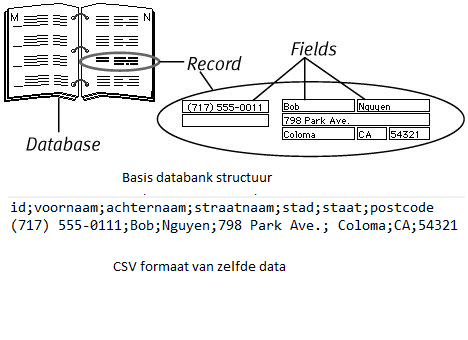
\includegraphics[width=\textwidth, height=\textheight, keepaspectratio]{databank_vs_CSV}
	\caption{Databank anatomie\cite{Hester2006} vs CSV structuur inhoud}
\end{figure}

\section{Datamining}

Datamining is een multidisciplinair gebied dat statistiek, databanktechnologie, patroonherkenning, machine learning, gegevensvisualisatie en expertise in systemen omvat.
Wanneer een onderzoek werkt met grote datasets, is het manueel nagaan van verbanden ingewikkeld en heeft de data dus als vereiste automatisch gecontroleerd te worden.
Datamining bestaat uit het onderzoeken van bestaande data uit grote bestaande databanken, met als doel nieuwe data te genereren. Datamining is eerder waardevol voor gecompliceerdere zoektermen, zoals "Welk verband kan gevonden worden tussen de verzekeringscontracten die afgesloten werden het voorbije jaar?".
Op zichzelf is datamining een proces waar, in een grote set data, onderzoek wordt gedaan naar nuttige, relevante data. Het vinden van patronen, algoritmes en afwijkingen in deze grote set data moeten hierbij helpen. Het doel van de datamining techniek is om net ongekende patronen te vinden in de set data om deze vervolgens met elkaar te kunnen linken en structureren. Dit kan dan een antwoord bieden op business gerelateerde vragen die te tijd consumerend zijn om zelf op te lossen. \autocite{osman2019data} In detail kan dit logisch proces is onderverdeeld in 2 delen: het wetenschappelijke en het commerciële. Voornamelijk zijn toepassingen die het dataminen bevorderen in de InsurTech voornamelijk gefocust op het commerciële. \autocite{hand2007principles}


\section{Webscraping vs Datamining}

Nu voorgaande termen onderling zijn besproken, wordt het verschil of de samenhang van beiden besproken. In het kort werd webscraping eerder omschreven als een data ophalen. Terwijl webscraping eerder het ophalen van data is en formatteren doet het geen analyse of dataprocessing. Het is net de datamining die de opgehaalde data zal verrijken en hieruit conclusies, verbanden en verschillen uit zal halen. In feite kan web scraping dus gebruikt worden om datasets te creeëren waarop datamining wordt toegepast. Deze beiden vullen elkaar dus aan. In het kort is web scraping dus het extraheren van data en is data mining het analyseren van (optioneel de geëxtraheerde) data.

\section{Google Developer Tools}
DevTools (~development tools) zijn programma's die een ontwikkelaar ondersteunen bij het maken van software. Deze tools zijn tegenwoordig gekoppeld aan de browser en worden dus vooral gebruikt bij het ontwikkelen van web applicaties. 
Zo laten deze tools toe om de software te maken, testen en debuggen.

De web applicatie kan worden geïnspecteerd via DevTools door gebruik te maken van de shortcut "F12" in Google Chrome. Wanneer men de DevTools opent, zijn er verschillende tabbladen beschikbaar. Dit zijn de meest relevante:
\begin{itemize}
	\item Elements: 
		Via dit tabblad kunnen alle HTML elementen (samen met hun CSS) van de webpagina bekeken worden. Deze elementen zullen door de webscraper gebruikt worden om de relevante data te extraheren.
	\item Console:
		Dit tabblad bevat de consolemeldingen die de webapplicatie genereert.
 	\item Sources:
		Hier zijn alle resources zichtbaar die werden geladen met de pagina. Hier kunnen bijvoorbeeld de javascript bestanden bekeken worden.
	\item Network:
		Het network tabblad bevat alle network requests die gebeurd zijn.
	\item Application: 
		Dit tabblad wordt gebruikt om web app manifesten, service workers, en service worker caches te inspecteren, wijzigen en debuggen.
\end{itemize}
Deze DevTools worden vaak door web ontwikkelaars gebruikt om HTML pagina's op te maken of wijzigingen uit te voeren en controleren.

\section{InsurTech mogelijkheden}

Niet alleen de FinTech heeft reeds doorbraken gehad op technologisch vlak die als een ware revolutie lijken. Eind de jaren 1900 werd de bankautomaat, die het mogelijk maakte na sluiting van de bank nog steeds geld af te halen, in België geïntroduceerd. Hoewel dit echter al een enorme stap in de digitale revolutie was, werd 2 decennia later de mobiele betalingstechnologie een noviteit. \autocite{agarwal2020real} Deze voorbeelden van mogelijkheden binnen de FinTech zijn niet de enige die efficiëntie van het bankieren bevorderen. Echter ligt de focus bij dit onderzoek op de mogelijkheden die reeds bestaan en nog kunnen bestaan in de InsurTech. De twee hoofdgebieden waar conservatieve en moderne verzekeringsmaatschappijen gerelateerd zijn betreffen data en consumenten. Door gebruik te maken van InsurTech mogelijkheden kunnen conservatieve verzekeraars nieuwe producten en diensten aanbieden, de verzekeringsdekking uitbreiden tot voorheen onderverzekerde marktgroepen, de verwerking van claims stroomlijnen, de transactiekosten verlagen, en zorgen voor een betere risicobeoordeling en -bewaking. Door de technologische ontwrichting staan de verzekeringsmaatschappijen steeds meer onder druk om hun klantgerichte procedures te moderniseren en te innoveren. De digitale knowhow van insurtech-bedrijven, waarvan de aanwezigheid eerder als een kans dan als een bedreiging moet worden gezien, zou op dit gebied een nuttige hulp kunnen zijn. Welke knowhow dit precies is en hoe deze wordt geïmplementeerd is deel van het onderzoek dat volgt. \autocite{koprivica2018insurtech}
